\subsection{Refactoring and Optimizations} \label{ssec:val_refactoring_and_optimizations}
The changes made described in Section \ref{ssec:refactoring_and_optimizations} brought a CPU time reduction much larger than anticipated, especially for the DCHB engine.
Contrasted to Figure \ref{fig:engines-times-sep2018}, where the time DCHB and DCTB took per event was $169.68$ [ms] and $47.76$ [ms] on average, the new times for each is $118.14$ [ms] and $44.34$ [ms] respectively, meaning an improvement of $30.1\%$ for DCHB and, less impressively, of $7.2\%$ for DCTB.

As shown in Figure \ref{fig:methods_times-1_1}, there are some differences in the percent of the total CPU time distributed on each engine, with a heavy reduction apparent in the \texttt{clusterSplitter} and \texttt{setFitArray} methods.
Using the versioning method mentioned in Section \ref{ssec:prof_results}, this version is named $1.1$.

    \begin{figure}[ht]
        \centering
        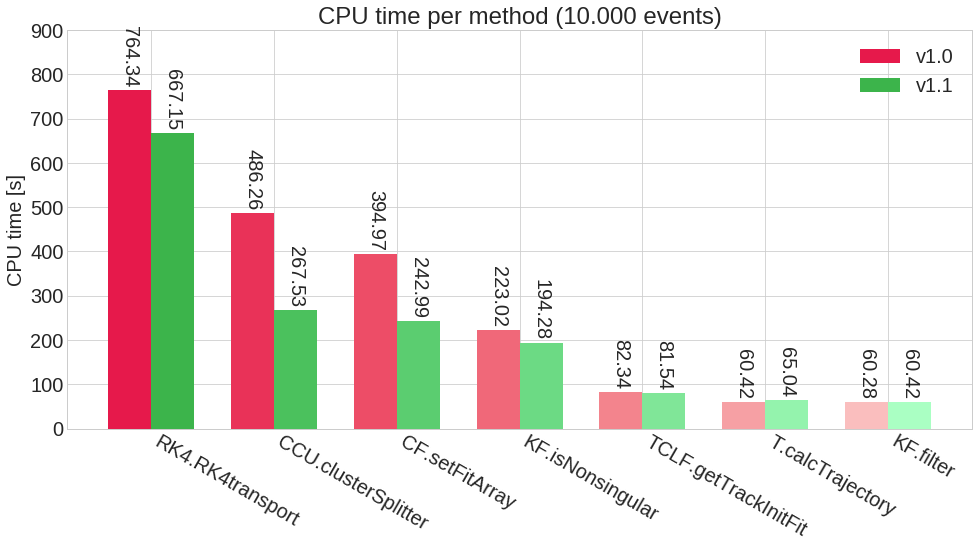
\includegraphics[scale=0.44]{methods_times/1_1}
        \caption{\label{fig:methods_times-1_1} CPU time per method, version $1.1$ contrasted with $1.0$.}
    \end{figure}

A comprehensive list of the improvements is presented:
\begin{itemize}
    \item \textbf{Runge Kutta 4}: The total reduction in the time spent in the \texttt{RK4transport} method was of a $12.7\%$ ($97.19$ seconds) for the $10.000$ events evaluated.
    This is attributed to the precomputation of values achieved via the refactoring of the code that was done after comparing the original code with the real Runge Kutta 4 algorithm.
    Since the original implementation makes very little use of the modularity inherent to the algorithm, the refactoring highlighted that the computations were done repeatedly since the new code is much shorter and easier to comprehend.

    \item \textbf{Cluster Splitter} and \textbf{Set Fit Array}: Both these methods were accelerated in a very similar manner to the one last described, reducing the total CPU time by $45.0\%$ (from $486.26$ to $267.53$ [s]) and by $38.5\%$ (from $394.97$ to $242.99$ [s]) respectively, thus making these two methods less of a priority when compared to RK4.
    
    \item \textbf{Is Nonsingular}: For this method a very small reduction in CPU time is perceived, just of $12.9\%$ (from $223.02$ to $194.28$ [s]) in total.
    No change was made to this method, so the reduction is associated to the addition of better exception handling in previous steps so that iterations with ``useless'' data are stopped before reaching this point in the computation.
    
    \item \textbf{Get Track's Initial Fit}, \textbf{Calculate Trajectory} and \textbf{Filter}: These methods' CPU time were preserved between versions, seeing only very minor change.
    This is attributed to the profiler's measurement error.
\end{itemize}